\documentclass[final,t,overlay, xcolor=table, sans, mathserif]{beamer}
\mode<presentation>
{
\usetheme{UCL}
}
\usepackage[orientation=landscape,size=a0,scale=1.15, debug]{beamerposter}
% \usepackage[orientation=landscape,size=custom, width=141, height=100,scale=1.2, debug]{beamerposter}
% \usepackage[orientation=landscape,size=custom,width=178,height=88.8,scale=1.6]{beamerposter}

% additional packages
\usepackage{tikz}
\usepackage{paralist}
\setdefaultleftmargin{4.5em}{}{}{}{}{}
\usepackage{array}
\usepackage[english]{babel}
\usepackage[latin1]{inputenc}
\usepackage{wrapfig}
\usepackage{amsmath}
\usepackage{natbib}
\usepackage{multirow}
%\usepackage[pdftex]{graphicx}
\usepackage{epstopdf} 
\usepackage{xcolor}
%\usepackage{svg}
%\usepackage[inkscape={/Applications/Inkscape.app/Contents/Resources/bin/inkscap??e -z -C}]{svg}

%\usepackage{kerkis}
%\usepackage{kmath}


% additional settings
\setbeamerfont{itemize}{size=\normalsize}
\setbeamerfont{itemize/enumerate body}{size=\normalsize}
\setbeamerfont{itemize/enumerate subbody}{size=\normalsize}

\pdfpageattr{/Group << /S /Transparency /I true /CS /DeviceRGB>>}


%\graphicspath{{fig/}}

% Display a grid to help align images
%\beamertemplategridbackground[1cm]

\title{Performance of synchrony and spectral-based features in early seizure detection:\\ exploring feature combinations and effect of latency.}
\author[Adam \& Soldado-Magraner]
{Vincent Adam$^1$, Joana Soldado Magraner$^1$, Wittawat Jitkrittum$^1$, Heiko Strathmann$^1$, Balaji Lakshminarayanan$^1$, Alessandro Davide Ialongo$^1$, Gergo Bohner$^1$, Ben Dongsung Huh$^1$,\\ Lea Goetz$^2$, Shaun Dowling$^3$, Iulian Vlad Serban$^3$, Matthieu Louis$^3$}
\institute[UCL]{The Gatsby Computational Neuroscience Unit$^1$, Wolfson Institute for Biomedical Research$^2$, The Centre for Computational Statistics and Machine Learning$^3$ (CSML), UCL, London, UK.}

\date[IWSP7 2015]{IWSP7 2015}


\begin{document}
\begin{frame}{}


\begin{columns}[t]
%%%%%%%%%%%%% BEGIN COLUMN ONE %%%%%%%%%%%%%%%%%%%%%%%%%%%%%%%%%%%%%%%%%%%%
\begin{column}{.35\linewidth}



\begin{block}{Motivation}
\end{block}



\begin{block}{Previous work on detection}
\begin{minipage}[t]{1\linewidth}
\end{minipage}
\end{block}

\begin{block}{Our algorithm}
\end{block}




\end{column}
%%%%%%%%%%%%% BEGIN COLUMN TWO %%%%%%%%%%%%%%%%%%%%%%%%%%%%%%%%%%%%%%%%%%%%
\begin{column}{.65\linewidth}

 
\begin{block}{The task}
\end{block}



\begin{columns}
\column{0.49\textwidth}
\begin{block}{Results I. Performance}
\begin{columns}
\column{0.49\textwidth}
\begin{figure}
\includegraphics[width=1\textwidth]{figures/kaggle_2_train_test_early.pdf}
\end{figure}
\column{0.49\textwidth}
\begin{figure}
\includegraphics[width=1\textwidth]{figures/kaggle_2_train_test_early.pdf}
\end{figure}
\end{columns}
\end{block}
\column{0.49\textwidth}
\begin{block}{Results II. Latency}
\centering
Mean performance across subjects, for different feature combinations.
\begin{figure}
\includegraphics[width=0.85\textwidth]{figures/all_latency.pdf}
\end{figure}
\end{block}
\end{columns}

\begin{columns}
\column{0.49\textwidth}
\begin{block}{Results II. Latency. Example 1.}
\begin{figure}
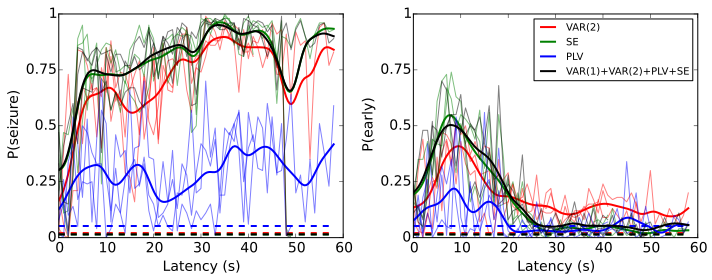
\includegraphics[width=0.85\textwidth]{figures/Patient_2_latency.pdf}
\end{figure}
\end{block}
\column{0.49\textwidth}
\begin{block}{Results II. Latency. Example 2.}
\begin{figure}
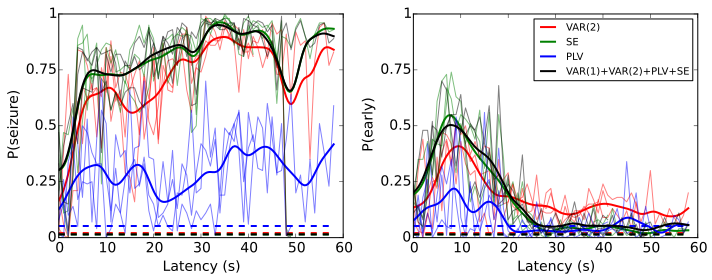
\includegraphics[width=0.85\textwidth]{figures/Patient_2_latency.pdf}
\end{figure}
\end{block}
\end{columns}




\begin{block}{Conclusions}
\end{block}




\end{column}
%%%%%%%%%%%%% END COLUMNS %%%%%%%%%%%%%%%%%%%%%%%%%%%%%%%%%%%%%%%%%%%%
\end{columns}


\end{frame}
\end{document}
